\chapter{ANOVA}
One-way ANOVA is a common procedure in statistics, and is related to the
simpler idea of a t-test. These classical tests were designed for particular
kinds of problems, and in this chapter we will study similar problems but
solve them from a Bayesian point of view.
We will also use these examples to discuss some issues about the choice
of prior distributions when there are more than a few parameters,
and to introduce the idea of a {\it hierarchical model}.

\section{A T-Test Example}
This example is based on one given in a 1976 article by physicist E. T. Jaynes,
called ``Confidence Intervals vs. Bayesian Intervals''. This is a very strongly
worded paper and might be an interesting read for
those who are interested in the battle between frequentist and Bayesian statistics
when the latter was making its comeback in the second half of the 20th century.
It's also where I got the crazy confidence interval example from.

Two manufacturers, $1$ and $2$, both make ``widgets'', and we are interested
in figuring out which manufacturer makes the best widgets (on average), as
measured by their lifetime. To determine this, we obtain 9 widgets from
manufacturer $1$ and 4 widgets from manufacturer $2$, and measure their
lifetimes, in days. The results are given below:
\begin{eqnarray}
x^1 &=& \{41.26, 35.81, 36.01, 43.59, 37.50, 52.70, 42.43, 32.52, 56.20\}\\
x^2 &=& \{54.97, 47.07, 57.12, 40.84\}
\end{eqnarray}
These measurements can be summarised by the means and standard deviations, which
are $42 \pm 7.48$ for group $1$ and $50 \pm 6.48$ for group $2$.
The question is: given this data, is there evidence that one of the manufacturers
is better than the other, and if so, by how much?
In classical statistics the standard procedure for this situation would be a
two sample $t$0-test. However, before we do anything I'd like you to consider
the numbers and use your intuition: what do {\it you} think about what the
evidence says?

An underlying assumption of a classical $t$-test is that the data are normally
distributed around the mean values for each group. We may as well adopt this
assumption for our Bayesian model. If we call the group 1
data points $\{x^1_1, x^1_2, ..., x^1_{N_1}\}$ and the group 2 data points
$\{x^2_1, x^2_2, ..., x^2_{N_1}\}$, then the likelihood is:
\begin{eqnarray}
x^1_i &\sim& \mathcal{N}\left(\mu_1, \sigma^2\right)\nonumber\\
x^2_i &\sim& \mathcal{N}\left(\mu_2, \sigma^2\right)\label{eq:ttest_likelihood}
\end{eqnarray}
Where all the data points are independent given the parameters. Note the assumption that
the two groups have the same underlying (``population'') standard deviation $\sigma$. This is a popular
assumption in this kind of analysis but it is not necessarily well justified!
We will build our Bayesian models using this assumption, but it is not that
difficult to relax it if you want to. You could just include multiple
$\sigma$ parameters in the model,
just like how we will include the multiple $\mu$ parameters.

Instead of just one model for this situation, we will study three different
versions. Each model will have the same likelihood
as given above in Equation~\ref{eq:ttest_likelihood}, and the same prior
for $\sigma$. However, the models will all have different priors for $\mu_1$
and $\mu_2$.
We will be able to see that the choice of prior does
influence the results (of course), but in ways that make sense. Which of these
models is more appropriate in a practical situation would depend on the exact
situation. There is no ``one size fits all'' model.

\subsection{Likelihood}
To implement our model in JAGS, we can begin by specifying the likelihood
part like so:

\begin{framed}
\begin{verbatim}
    # Sampling distribution/likelihood
    for(i in 1:N1)
    {
        x1[i] ~ dnorm(mu1, 1/sigma^2)
    }
    for(i in 1:N2)
    {
        x2[i] ~ dnorm(mu2, 1/sigma^2)
    }
\end{verbatim}
\end{framed}
We have called our data arrays {\tt x1} and {\tt x2}, and we have also
assumed that the sample sizes {\tt N1} and {\tt N2} are defined, so our
{\tt data} list will need to be consistent with these choices. The parameters
we will be estimating are {\tt mu1}, {\tt mu2}, and {\tt sigma}, so we will
need to specify prior distributions for them. In the following sections, we'll
use the same prior for {\tt sigma}, so we may as well specify that now.
Let's use a log-uniform prior.

\begin{framed}
\begin{verbatim}
    # Prior for sigma
    log_sigma ~ dunif(-10, 10)
    sigma <- exp(log_sigma)
\end{verbatim}
\end{framed}

\subsection{Prior 1: Very Vague}
The last missing ingredient to finish the JAGS model are the priors for
{\tt mu1} and {\tt mu2}. For our first model, let's be really naive and assign
super-wide uniform priors.

\begin{framed}
\begin{verbatim}
    # Prior 1: Very Vague
    mu1 ~ dunif(-1000, 1000)
    mu2 ~ dunif(-1000, 1000)
\end{verbatim}
\end{framed}


\subsection{Prior 2: They might be equal!}

\begin{framed}
\begin{verbatim}
# Actually allow mu1=mu2
model
{
    # Log-uniform prior for the amount of scatter
    log_sigma ~ dunif(-10, 10)
    sigma <- exp(log_sigma)

    # First mean
    mu1 ~ dnorm(0, 1/1000^2)

    # Prior on second mean
    difference ~ dt(0, 1/5^2, 1)
    flag ~ dunif(0, 1)
    mu2 <- mu1 + difference*step(flag - 0.5)

    # Sampling distribution/likelihood
    for(i in 1:N1)
    {
        x1[i] ~ dnorm(mu1, 1/sigma^2)
    }
    for(i in 1:N2)
    {
        x2[i] ~ dnorm(mu2, 1/sigma^2)
    }
}
\end{verbatim}
\end{framed}

\subsection{Prior 3: Alright, they're not equal, but they might be {\it close}}

The results of the three different models are shown below:
\begin{figure}
\begin{center}
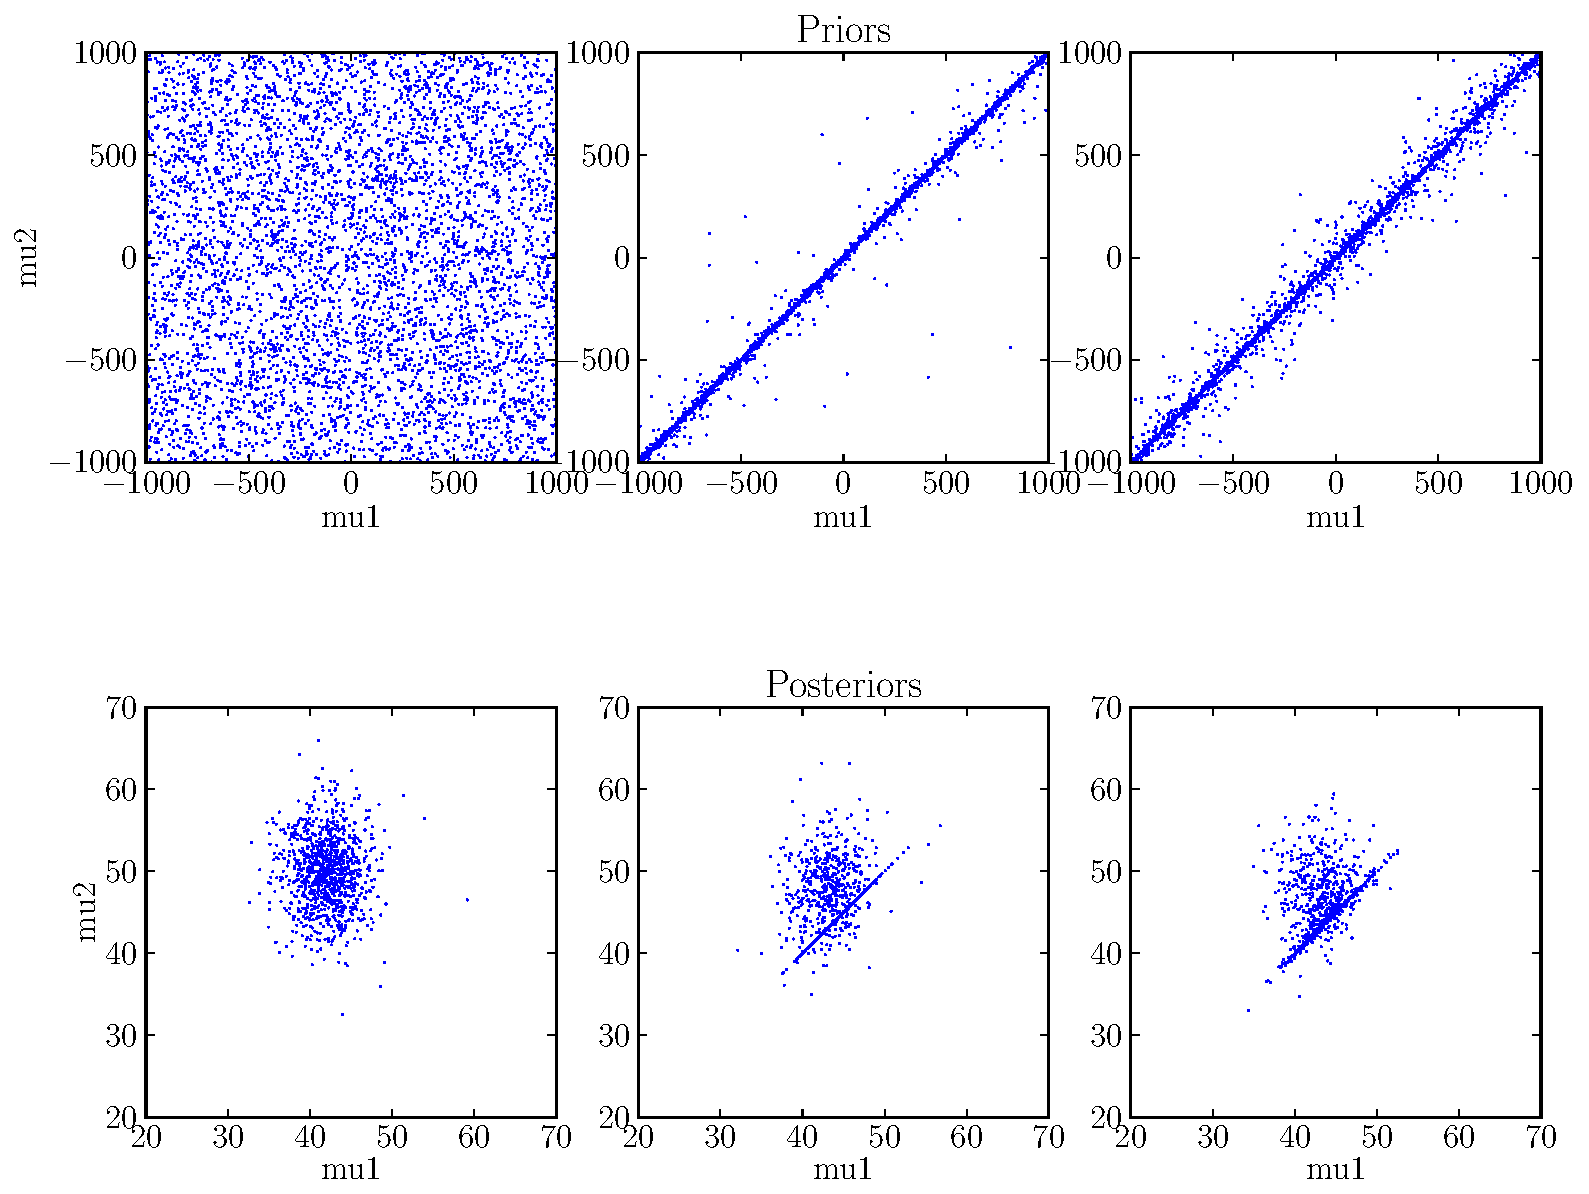
\includegraphics[scale=0.6]{Figures/ttest.pdf}
\end{center}
\end{figure}


\section{One Way Anova}
One-way ANOVA can be considered as a generalisation of a t-test to more than
two groups. The question is usually phrased as a test of the hypothesis that
the group means are the same, versus the alternative that there is some difference.
As we saw in the Bayesian ``t-test'', it is possible (using clever tricks) to
make a model that has some prior probability that the group means are equal.
However, this gets more tricky with multiple groups. Therefore we will build our
one-way ANOVA model in a similar way to the ``hierarchical model'' version of the
t-test model. There will be one other major difference, but it is a difference
in the way the model is coded, not a conceptual difference. In the t-test
section we used different 

The masses of starlings were measured at four locations.

\begin{figure}[ht!]
\begin{center}
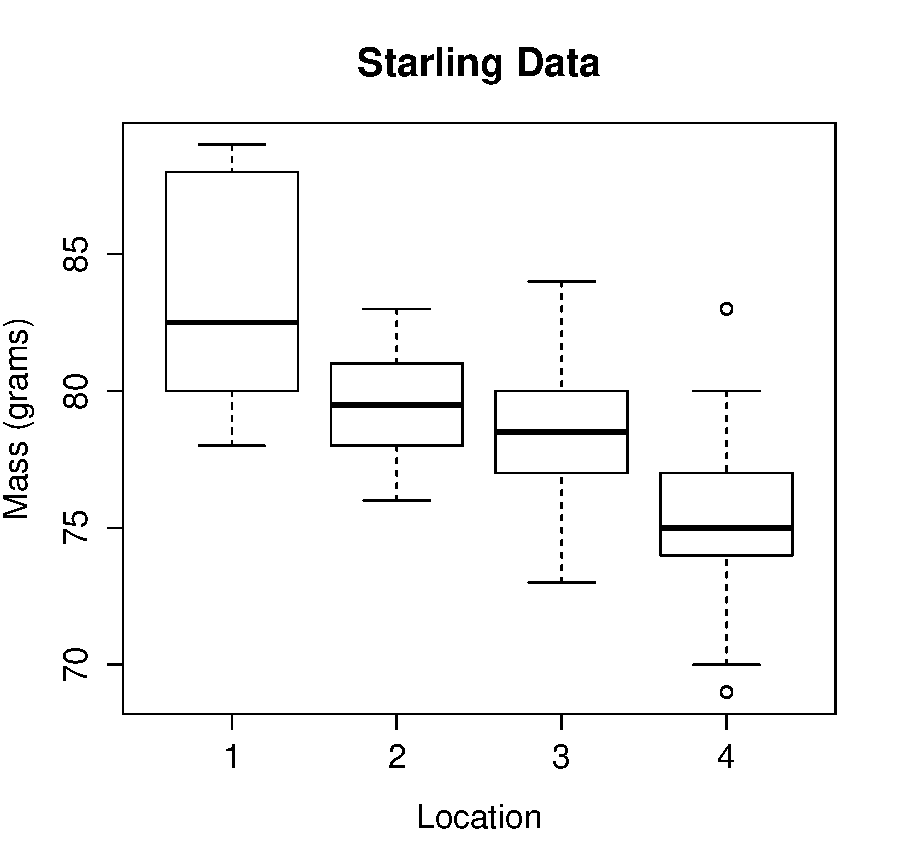
\includegraphics[scale=0.6]{Figures/starling.pdf}
\end{center}
\end{figure}


\subsection{Hierarchical Model}
The main advantage of this model is that it generalises to more than two groups
in a very straightforward way. The difference is the prior. Whereas the first
model had independent priors for the means of the groups, this version is our
first example of a {\it hierarchical model}.
\begin{framed}
\begin{verbatim}
model
{
    # Log-uniform prior for the scatter
    log_sigma ~ dunif(-10, 10)
    sigma <- exp(log_sigma)

    # Hierarchical prior for the means
    # Hyperparameters
    grand_mean ~ dnorm(0, 1/1000^2)
    log_diversity ~ dunif(-10, 10)
    diversity <- exp(log_diversity)

    # Parameters
    mu1 ~ dnorm(grand_mean, 1/diversity^2)
    mu2 ~ dnorm(grand_mean, 1/diversity^2)

    # Sampling distribution/likelihood
    for(i in 1:N)
    {
        x[i] ~ dnorm(mu[group[i]], 1/sigma^2)
    }
}

\end{verbatim}
\end{framed}


